\label{sec:demo}
%%%%%%%%%%%%%%%%%%%%%%%%
In order to show the capabilities introduced with the new DET module, a simplified PWR Dynamic PRA analysis is here presented.
\begin{figure}[h]
   \centering
    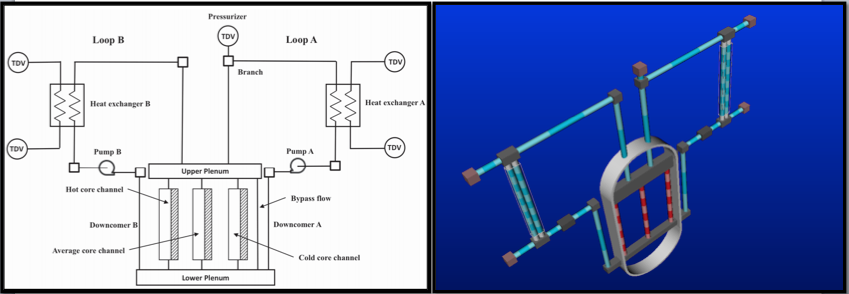
\includegraphics[width=1.0\textwidth]{figures/PWR_TMI_SCHEME.PNG}
    \caption{PWR model scheme}
    \label{fig:PWRmodel}
\end{figure}
Figure~\ref{fig:PWRmodel} shows the scheme of the PWR model. The reactor vessel model consists of the Down-comers, the Lower Plenum, the Reactor Core Model and the Upper Plenum. Core channels (flow channels with heat structure attached to each of them) are used to describe the reactor core. The core model consists of three parallel core channels and one bypass flow channel.
%The hot core channel represents the inner hottest zone of the reactor core. The average core channel represents the mid zone of the core and the cold core channel represents the outer zone of the core, respectively.
There are two primary loops, i.e., loop A and loop B. Each loop consists of the Hot Leg, a Heat Exchanger and its secondary side pipes, the Cold Leg and a primary Pump. A Pressurizer is attached to the Loop A piping system to control the system pressure. A Time Dependent Volume (pressure boundary conditions) component is used to represent the Pressurizer. Since the RELAP-7 code two-phase flow capability has not being used for this test, single-phase counter-current heat exchanger models are implemented to mimic the function of steam generators in order to transfer heat from the primary to the secondary.

In order to perform a DPRA analysis of this simplified model, it has been necessary to control unconventional parameters (i.e. inlet/outlet friction factors), since RELAP-7 still has limitations for the component controllable parameters and models. In the following paragraph, the PRA station black out sequence of events is reported.
%%%%%%%%%%%%%%%%%%%%%%%%%%%%%%
\subsection{Station Black Out (SBO) analysis}
%%%%%%%%%%%%%%%%%%%%%%%%%%%%%%
\label{sec:SBOanalysis}
The simulation of a SBO initiating event required the introduction, in the control logic, of several components (see Fig.~\ref{fig:SchemeElSystem}):
\begin{figure}[h]
   \centering
    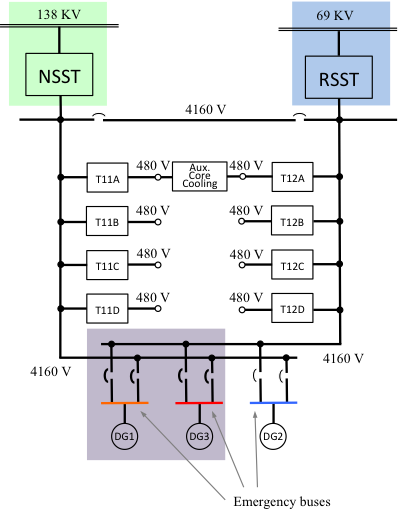
\includegraphics[width=0.4\textwidth]{figures/SchemeEletricalSystem.png}
    \caption{Scheme of the electrical system of the PWR model}
    \label{fig:SchemeElSystem}
\end{figure}

\begin{itemize}
\item Set of 3 diesel generators (DGs) and associated emergency buses
\item Primary power grid line 138 KV (connected to the NSST switchyard)
\item Auxiliary power grid line 69 KV (connected to the RSST switchyard)
\item Electrical buses: 4160 V (step down voltage from the power grid and voltage of the electric converter connected to the DGs) and 480 V for actual reactor components (e.g., reactor cooling system)
\end{itemize}
The scenario is the following:
\begin{itemize}
\item An external event causes a loss of off-site power (LOOP) due to damage of the 138 kV line and RSST switchyard; the reactor successfully scrams and, thus, power generated in the core follows the characteristic exponentially decay curve
\item The set of DGs fails to start and, hence, conditions of SBO are reached (4160 V and 480 V buses are not energized); all cooling systems are subsequently off-line
\item Without the ability to cool the reactor core, its temperature starts to rise
\item In order to recover AC electric power on the 4160 V and 480 V buses, two recovery teams are assembled with the following strategy:
\begin{itemize}
\item Recovery Team 1 focuses on the recovery of the DGs: due to internal damage at the DG building, two DGs (i.e., DG1 and DG3) need to be repaired (see Fig.~\ref{fig:ACPowerRecovery}~(a))
\item Recovery Team 2 focuses on the recovery of the RSST switchyard; 69KV line is energized but the RSST switchyard needs to be recovered (see Fig.~\ref{fig:ACPowerRecovery}~(b))
\end{itemize}
\item Meanwhile the owning company is working on the restoration of the primary 138 KV line (see Fig.~\ref{fig:ACPowerRecovery}~(c))
\item When the 4160 V buses are energized (through the recovery of the DGs, RSST or 138KV line), the auxiliary cooling system is able to cool the reactor core and, thus, core temperature decreases.
\end{itemize}

\begin{figure}
        \centering %
        ~ %add desired spacing between images, e. g. ~, \quad, \qquad etc.
          %(or a blank line to force the subfigure onto a new line)
        \begin{subfigure}[b]{0.3\textwidth}
                \centering
                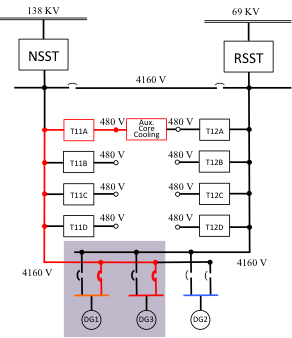
\includegraphics[width=\textwidth]{figures/ACpowerRecPathDGs.png}
                \caption{}
                \label{fig:ACpowerDGs}
        \end{subfigure}
        \begin{subfigure}[b]{0.3\textwidth}
                \centering
                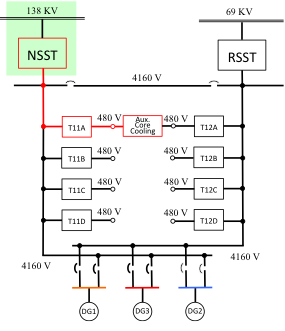
\includegraphics[width=\textwidth]{figures/ACpowerRecPath138kV.png}
                \caption{}
                \label{fig:ACpower138kV}
        \end{subfigure}
        ~ %add desired spacing between images, e. g. ~, \quad, \qquad etc.
          %(or a blank line to force the subfigure onto a new line)
        \begin{subfigure}[b]{0.3\textwidth}
                \centering
                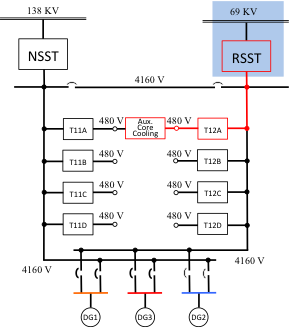
\includegraphics[width=\textwidth]{figures/ACpowerRecPathRSST.png}
                \caption{}
                \label{fig:ACpowerRSST}
        \end{subfigure}
        \caption{AC power recovery paths through: DGs (a), RSST (b) and 138KV line (c). Red lines indicate electrical path to power Auxiliary cooling system}\label{fig:ACPowerRecovery}
\end{figure}

Given the uncertainties associated to the recovery of both DGs, RSST and 138KV line, a stochastic model has been used to represent these events . Given the time scale associated to the dynamics of the RELAP-7 PWR model the corresponding probability distribution functions were as follows:
\begin{itemize}
\item DGs: a dead time of 100s is required by Team 1 to gather at the DGs building and DG1 repair time $TDG1$ has a normal distribution having mu = 800 and sigma = 200. This distribution is also truncated such that $0 < TDG1 < 2500$. The recovery time of DG3, TDG3 , is proportional to $TDG1$. Such relation has modeled using a multiplication factor T12, i.e., $TDG3 = TDG1\times T12$. T12 is uniformly distributed between [0.5 1]
\item RSST: a dead time of 400s is needed to assess the damage at the RSST switch-yard and to plan its recovery. Recovery time for RSST, TRSST , is normally distributed with mu = 1400 and sigma= 400
\item 138KV line: the recovery of the main AC line T138 is normally distributed with mu = 2000 and sigma = 500
\end{itemize}

In addition, the clad failure temperature $T_{C,fail}$ is not fixed but it is probabilistic distributed with a triangular distribution with the following parameters:
\begin{itemize}
\item mode: xPeak = 1477.59 K, 10CFR regulatory limit
\item lower bound: xMin = 1255.37 K, PRA success criterion
\item upper bound: xMax = 1699.82 K, Urbanic-Heidrick transition temperature ~\cite{Urbanic1978}
\end{itemize}

%%%%%%%%%%%%%%%%%%%%%%%%%%%%%%

The DET calculation has been run considering equally spaced branching probability thresholds (ESBP).

\begin{figure}
        \centering %
        ~ %add desired spacing between images, e. g. ~, \quad, \qquad etc.
          %(or a blank line to force the subfigure onto a new line)
        \begin{subfigure}[b]{0.48\textwidth}
                \centering
                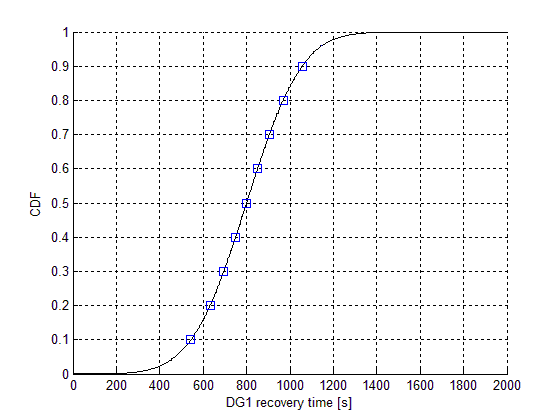
\includegraphics[width=\textwidth]{figures/DG1Dist.png}
                \caption{}
                \label{fig:DG1Dist}
        \end{subfigure}
        \begin{subfigure}[b]{0.48\textwidth}
                \centering
                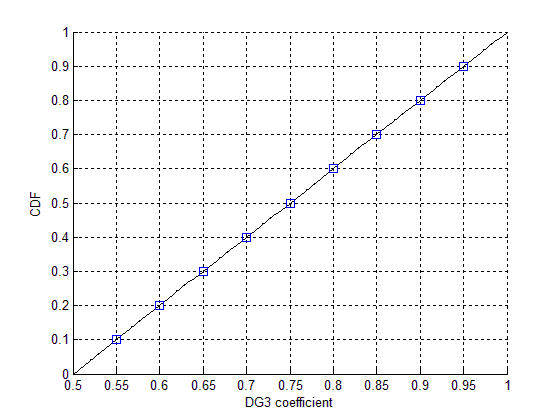
\includegraphics[width=\textwidth]{figures/DG3CoeffDist.png}
                \caption{}
                \label{fig:DG3CoeffDist}
        \end{subfigure}
        ~ %add desired spacing between images, e. g. ~, \quad, \qquad etc.
          %(or a blank line to force the subfigure onto a new line)
        \caption{Cumulative Distribution Functions and DET bins: (a) DG1, (b) DG3 coefficients}\label{fig:CDFsDGs}
\end{figure}
\begin{figure}
        \centering %
        ~ %add desired spacing between images, e. g. ~, \quad, \qquad etc.
          %(or a blank line to force the subfigure onto a new line)
        \begin{subfigure}[b]{0.48\textwidth}
                \centering
                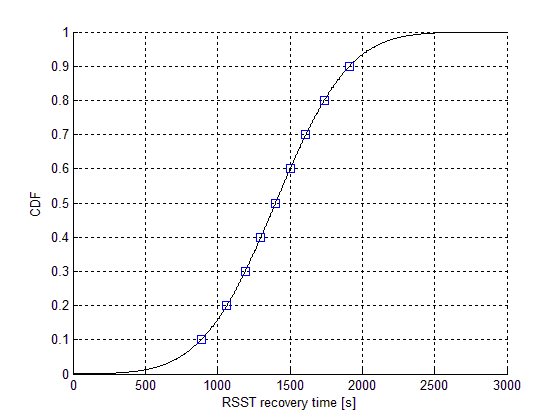
\includegraphics[width=\textwidth]{figures/RSSTDist.png}
                \caption{}
                \label{fig:RSSTDist}
        \end{subfigure}
        \begin{subfigure}[b]{0.48\textwidth}
                \centering
                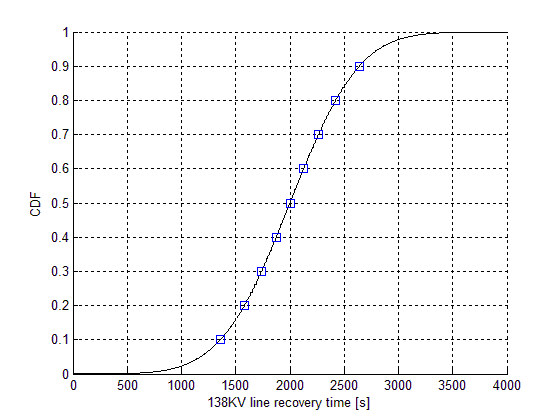
\includegraphics[width=\textwidth]{figures/138kVlineDist.png}
                \caption{}
                \label{fig:138kVlineDist}
        \end{subfigure}
        ~ %add desired spacing between images, e. g. ~, \quad, \qquad etc.
          %(or a blank line to force the subfigure onto a new line)
        \caption{Cumulative Distribution Functions and DET bins: (a) 138kV line, (b) RSST}\label{fig:CDFsACs}
\end{figure}
\begin{figure}
        \centering %
        ~ %add desired spacing between images, e. g. ~, \quad, \qquad etc.
          %(or a blank line to force the subfigure onto a new line)
        \begin{subfigure}[b]{0.48\textwidth}
                \centering
                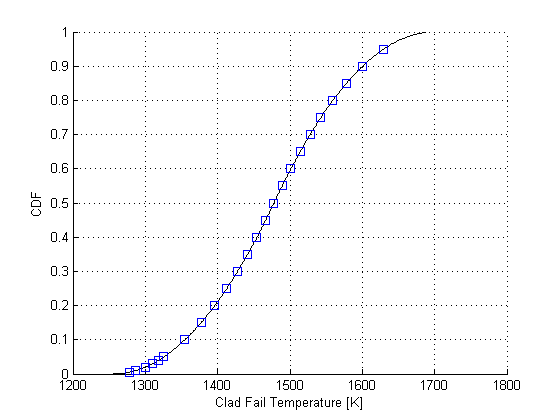
\includegraphics[width=\textwidth]{figures/CladFailureDist.png}
                \caption{}
                \label{fig:CladFailure}
        \end{subfigure}
        \caption{Cumulative Distribution Function and DET bin for Clad Failure Temperature Distribution}\label{fig:CDFCladFailure}
\end{figure}
The probability threshold values are reported below:
\vspace{-5mm}
   \begin{itemize}
       \item DG1 recovery time distribution (Fig.~\ref{fig:CDFsDGs}~(a) - blue points):
       \begin{itemize}
            \item Probability Thresholds: 0.1, 0.2, 0.3, 0.4, 0.5, 0.6, 0.7, 0.8,  0.9
            \item Variable Values (s)           : 543.69 , 631.68, 695.12, 749.33, 800.00, 850.67, 904.88, 968.32, 1056.31
       \end{itemize}
       \item DG3 recovery factor distribution (Fig.~\ref{fig:CDFsDGs}~(b) - blue points):
       \begin{itemize}
            \item Probability Thresholds: 0.1, 0.2, 0.3, 0.4, 0.5, 0.6, 0.7, 0.8,  0.9
            \item Variable Values (-)           : 0.55, 0.60, 0.65, 0.70, 0.75, 0.80, 0.85, 0.90, 0.95
       \end{itemize}
       \item RSST recovery time distribution (Fig.~\ref{fig:CDFsACs}~(a) - blue points):
       \begin{itemize}
            \item Probability Thresholds:  0.1, 0.2,  0.3,  0.4, 0.5, 0.6, 0.7,  0.8,  0.9
            \item Variable Values (s)           :  887.38, 1063.35, 1190.24, 1298.66, 1400.00, 1501.34, 1609.76, 1736.65, 1912.62
       \end{itemize}
       \item 138 kV line recovery time distribution (Fig.~\ref{fig:CDFsACs}~(b) - blue points):
       \begin{itemize}
            \item Probability Thresholds: 0.1, 0.2, 0.3, 0.4, 0.5, 0.6, 0.7, 0.8, 0.9
            \item Variable Values (s)           : 1359.22,  1579.19,  1737.80, 1873.33,  2000.00,  2126.67, 2262.20,  2420.81, 2640.78
       \end{itemize}
       \item Clad Failure Temperature distribution (Fig.~\ref{fig:CDFCladFailure} - blue points):
       \begin{itemize}
            \item Probability Thresholds: 0.005, 0.01, 0.02, 0.03, 0.04, 0.05, 0.10, 0.15, 0.2, 0.25, 0.3, 0.35, 0.4, 0.45, 0.5, 0.55, 0.60, 0.65, 0.70, 0.75, 0.80, 0.85, 0.90, 0.95
            \item Variable Values (K)           : 1304.57, 1307.51, 1313.27, 1318.89, 1324.38, 1329.37, 1354.78, 1376.74, 1395.86, 1412.68, 1427.70, 1441.33, 1453.96, 1465.94, 1477.60, 1489.26, 1501.24, 1513.87, 1527.50, 	1542.51, 1559.34, 1578.45, 1600.40, 1625.79
    \end{itemize}
\end{itemize}
\vspace{-5mm}

Since the scope of this demo is to show the new capabilities contained in RAVEN, and RELAP-
7 is not optimized for long simulation times, the transient has been accelerated in order to reach a reasonable number of failures at of 2500 seconds.  In the following section, the simulations results are shown and discussed.
%%%%%%%%%%%%%%%%%%%%%%%%%%%%%%
\subsection{Results}
%%%%%%%%%%%%%%%%%%%%%%%%%%%%%%
DET analysis has been performed, obtaining a data-set composed by 593 DET branches resulting in 290 complete histories.

\begin{figure}
 \begin{minipage}[b]{8.5cm}
   \centering
   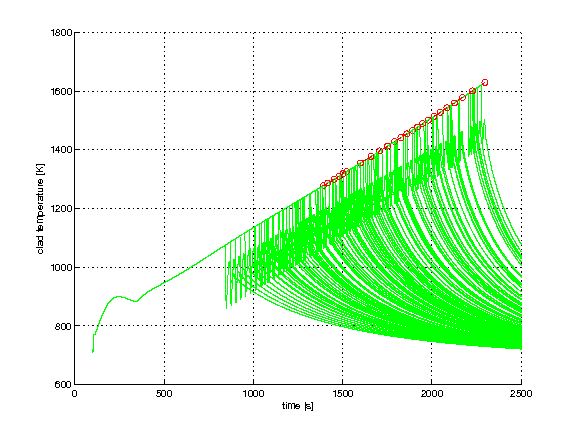
\includegraphics[width=9cm]{figures/CladTemperature.png}
   %\caption{Clad Temperature evolution in hot core channel.}
   %\label{fig:DETpbClad}
 \end{minipage}
 \ \hspace{2mm} \hspace{3mm} \
 \begin{minipage}[b]{8.5cm}
   \centering
   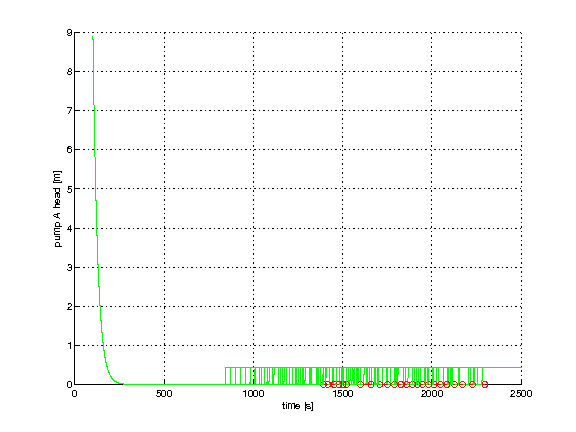
\includegraphics[width=9cm]{figures/HeadPump.png}
   %\caption{Pump Head evolution.}
   %\label{fig:DETpbHead}
 \end{minipage}
\caption{Clad Temperature (Left) and Pump Head (Right) temporal profiles (all histories)}
\label{fig:ESBPall}
\end{figure}
\vspace{-5mm}

Figure~\ref{fig:ESBPall} shows the histories obtained for the calculation performed.
Following the station back-out condition, the pump head decreases (pump coast-down) and the temperature of the core rises since reactor core cooling is not available. Such temperature increasing continues until one of the following conditions occurs:
\vspace{-5mm}
\begin{itemize}
\item Temperature of the clad reaches the clad failure temperature, indicated with a red circle (red scenarios in Fig.~\ref{fig:ESBPall}, or,
\item Auxiliary cooling system is restored (green scenarios in Fig.~\ref{fig:ESBPall}).
\end{itemize}
\vspace{-5mm}

Note that the back up of the cooling system causes oscillations on the clad temperature. These oscillations are determined by the sudden insertion of the auxiliary system that imposes a mass flow rate ~ 5\% of the operational one. The initial local maximum is due to the sudden loss of heat sink while the fuel still behaves as a heat reserve; after a while the remaining cooling capacity (pumps’ inertia) succeeds in reducing the temperature. The situation inverses again when the primary and secondary pumps completely stop.

From a safety point of view, the most important information is the frequency of failures in the phase space. This information can be shown plotting the final outcome (green points for system success and red points for system failure) of all the simulations for each data sets in a $2$-dimensional space. Since the DET sampling has been performed on 5 distributions, among which 4 distributions sampled the same parameter $ACS$ (Auxiliary Cooling System) Recovery Time, it is possible to collapse all the outcomes in a 2D space (ACS recovery time vs. clad failure temperature) as shown in Fig.~\ref{fig:LimitSurfaces}~(a).
The limit surface, i.e. the boundary between system failure and system success regions (black line), is also indicated in Fig.~\ref{fig:DET_LS}. Such boundary was determined using a Support Vector Machine (SVM) based algorithm~\cite{mandelliANS_RISMC}.
Note that most of the points in this $2$-dimensional space (for both data sets) lie in proximity  of the limit surface while samples generated by a classical Monte-Carlo based algorithm would be evenly distributed (see Fig.~\ref{fig:LimitSurfaces}~(b)).
This example shows one of the advantages of DET algorithm in terms of ``choosing" the best set of candidate samples when performing PRA analyses~\cite{alfonsiPSA}.

%%%%%%%%%%%%%%%%%
\begin{figure}
        \centering %
        ~ %add desired spacing between images, e. g. ~, \quad, \qquad etc.
          %(or a blank line to force the subfigure onto a new line)
        \begin{subfigure}[b]{0.48\textwidth}
                \centering
                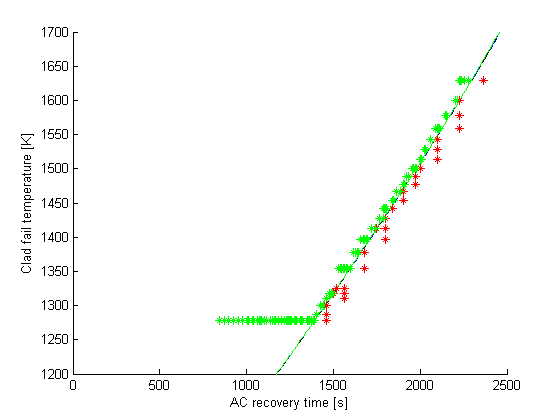
\includegraphics[width=\textwidth]{figures/limitSurface.png}
                \caption{}
                \label{fig:DET_LS}
        \end{subfigure}
        \begin{subfigure}[b]{0.48\textwidth}
                \centering
                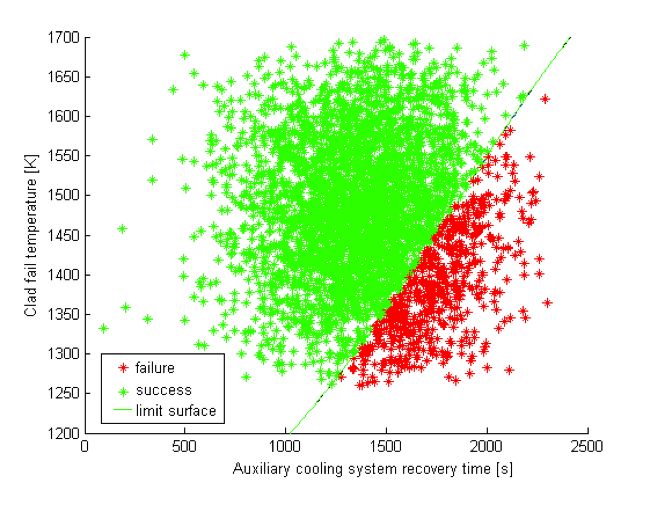
\includegraphics[width=\textwidth]{figures/MClimitSurface.png}
                \caption{}
                \label{fig:MonteCarloLS}
        \end{subfigure}
        ~ %add desired spacing between images, e. g. ~, \quad, \qquad etc.
          %(or a blank line to force the subfigure onto a new line)
        \caption{Limit Surfaces: (a) Dynamic Event Tree, (b) Monte-Carlo}\label{fig:LimitSurfaces}
\end{figure}

%Figure~\ref{fig:distributionResults} shows the distribution of the maximum temperature reached by the clad in the core channels (blue histogram) and compares it with the distribution of clad failure temperature (red histogram).
%Although there is large overlapping of the two distributions, which indicates a high failure probability of the system considered, the scope of the analysis was just to show  RAVEN capabilities to perform stochastic analysis of relatively complex systems.
%The distribution of the clad temperature already accounts for the simulations that have been stopped for having reached the corresponding failure temperature. Therefore, the overlapping of the two distributions is not representative of the total failure rate. Instead, the total failure rate could be inferred from the steep decrease on the higher temperature side of the number of counts with respect the lower temperature one. The probability of failure is artificially elevated with respect a real case in order to keep the effort bounded while illustrating the full RAVEN capabilities.
